%https://www.integral-domain.org/lwilliams/Resources/TikzImg/cubelattice2.tex
\documentclass[tikz]{standalone}

\definecolor{lgrey}{rgb}{0.7,0.7,0.7}
\begin{document}
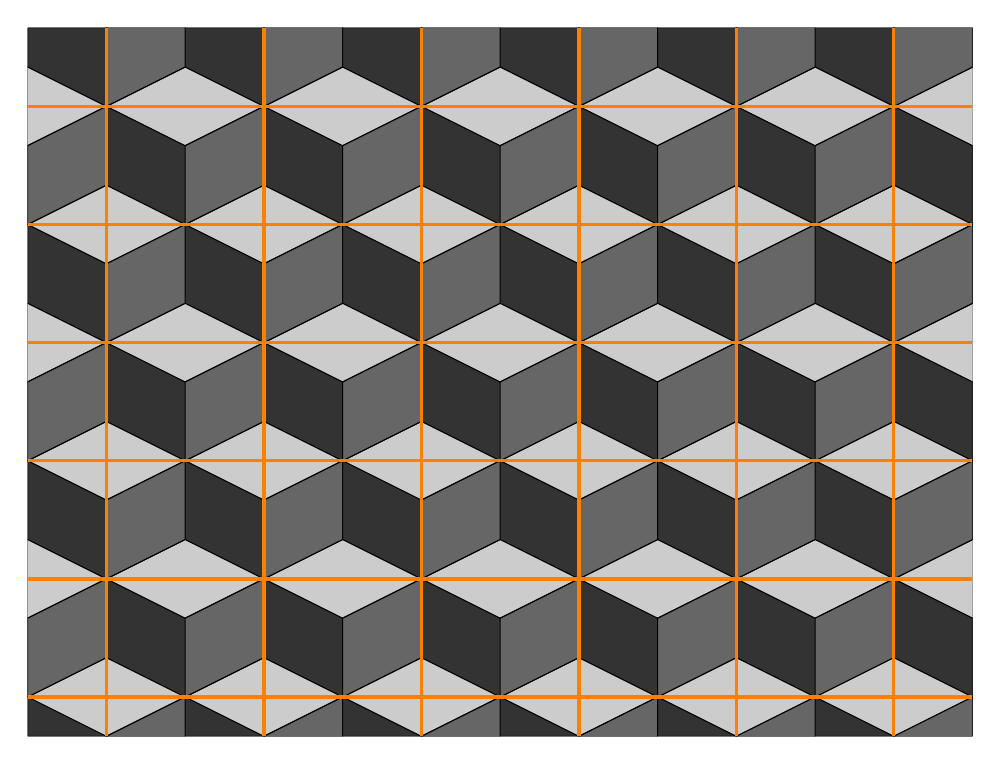
\begin{tikzpicture}[scale=1,y={(-1cm,0.5cm)},x={(1cm,0.5cm)}, z={(0cm,1cm)}]

% trim canvas, using isometric coordinates
\clip (0,1,-0.5)--(0,1,8.5)--(11,0,3.5)--(11,0,-5.5)--cycle;

% fill canvas, will be one of three visible colors
\draw[fill=black!80!white] (0,1,-0.5)--(0,1,8.5)--(11,0,3.5)--(11,0,-5.5)--cycle;

\foreach \y in {0,1,...,10} {   % rows
    \ifodd\y  % stagger columns in alternate rows
        \def\shift{-1cm}
    \else
        \def\shift{0cm}
    \fi
    \foreach \x in {0,1,...,10} { % columns
        \begin{scope}[ xshift=\x*2cm+\shift, yshift=\y*1.5cm ]
            \draw[fill=black!20!white] (0,0,0)--(1,0,0)--(1,1,0)--(0,1,0)--cycle;
            \draw[fill=black!60!white] (0,0,0)--(1,0,0)--(1,0,-1)--(0,0,-1)--cycle;
        \end{scope}
    }
}

        \foreach \x in {0,1,2,3,4,5}
            \draw[very thick, orange] (\x,-\x,0)--(\x,-\x,9);

        \foreach \z in {0,1.5,3,4.5,6,7.5}
            \draw[very thick, orange] (0,1,\z)--(6,-5,\z);


        \begin{scope}[xshift=14cm,yshift=3cm]
            \draw[fill=black!20!white] (0,0,0.5)--(0,0,1)--(1,0,0)--cycle;
            \draw[fill=black!20!white] (2,0,-0.5)--(2,0,0)--(1,0,0)--cycle;
            \draw[fill=black!20!white] (0,0,2)--(2,0,1)--(1,0,1)--cycle;

            \draw[fill=black!40!white] (1,0,0)--(2,0,0)--(0,0,2)--(0,0,1)--cycle;

            \draw[fill=black!80!white] (1,0,0)--(2,0,0)--(2,0,1)--(1,0,1)--cycle;

            \draw[very thick, orange] (0,0,0.5)--(2,0,-0.5)--(2,0,1)--(0,0,2);
        \end{scope}
    \end{tikzpicture}
 \end{document}